\section{Scalably Feasible QoI Regions}
\label{sec:scal_feasible_qoi}

In some applications, the data requirements to achieve a certain level of QoI may include a minimum number of nodes or sources in addition to the size of the data load that must be served.  For example, a system may require that each image must come from a different node, perhaps because each node only has one image or maybe by design to provide increased credibility through corroboration, another contextual metric of interest in QoI-aware networks.  We will use this example to illustrate an interesting observation that arises in such scenarios.
% may imply that a certain number of nodes afre required to achieve a desired level of QoI.  For example, a system may require $k_{req}$ images from $n$ different nodes.  

%Now let us consider a special case where nodes collect a total of $k_{req}$ images, but each image must come from a different node, perhaps because each node only has one image or maybe by design to provide increased credibility through corroboration, another contextual metric of interest in QoI-aware networks. This scenario allows us to illustrate an interesting observation.  

Let us assume that we are designing a surveillance network with nodes arranged in a grid and one data sink in the corner of the network.  This data sink node issues queries with a set of QoI requirements that include completeness and timeliness, $\mathbf{q} = \{C,T\}$, but this completeness must be met while only allowing one image per source node.  With this traffic model, we can derive a maximum traffic factor and create a scalability equation for this particular scenario.

Here, the data sink node will have two neighbors through which all queries will be forwarded, so clearly we can choose either of these to consider as the bottleneck node.  Even if the network balances traffic evenly over both of these nodes, each must forward at least $\frac{N-1}{2}-1$ since there are $N-1$ sources, half of which must be forwarded through each of the data sink's two neighbors, excluding the $1$ image from each of these neighbors themselves.  If we assume these queries may be simultaneously served in the worst case, then we can simply use this expression for the maximum Traffic Factor.  Then, using the same values derived for a grid network in Table \ref{table:rf_ff_sf_values} in place of the other factors in Equation (\ref{eq:general_scal}), we get the following scalability equation:

\begin{equation}
\setcounter{equation}{11}
	W \cdot T - 5 \cdot I_s \cdot (\frac{N-1}{2}-1) - 2.5 \cdot P_s \cdot 2 \sqrt{N} \geq 0
\end{equation}

%Consider a set of QoI requirements that include completeness and timeliness, $\mathbf{q} = \{C,T\}$.  As previously noted, a certain number of images are required to achieve this desired level of completeness, $Q(C) = k_{req}$.  Unlike the model used in Section \ref{sec:network_design}, however, each node can contribute only one image to $k_{req}$, which implies a minimum network size of $N \geq k_{req}$ in order to achieve the completeness outlined in the QoI requirements.  On the other hand, applying derived scalability equations to this network, we can determine the maximum network size, which we will call $N_{max}$ here for distinction.  
From this equation, we can determine the maximum network size, which we will call $N_{max}$ here.  However, the specified restriction that each node can contribute only one image to $k_{req}$ implies a minimum network size of $N \geq k_{req}$ in order to achieve the completeness outlined in the QoI requirements. 

These two facts are important, because when $N_{max} < k_{req}$, then it is not possible to provide the QoI level $\mathbf{q}$.  Hence, this set of QoI requirements is infeasible, or \emph{scalably infeasible}.  This phenomenon defines the concept of a \emph{Scalably Feasible QoI Region}, which refers to the region in which sets of QoI pairs can be supported with the given network signature.  

\begin{figure}[ht]
\centering
	\subfigure[The curved plane represents maximum scalability, and the flat plane represents minimum required images.  Therefore, all (Sum Sim., Timeliness) pairs to the right of the intersecting red line are within the scalably feasible QoI region.]
	{
		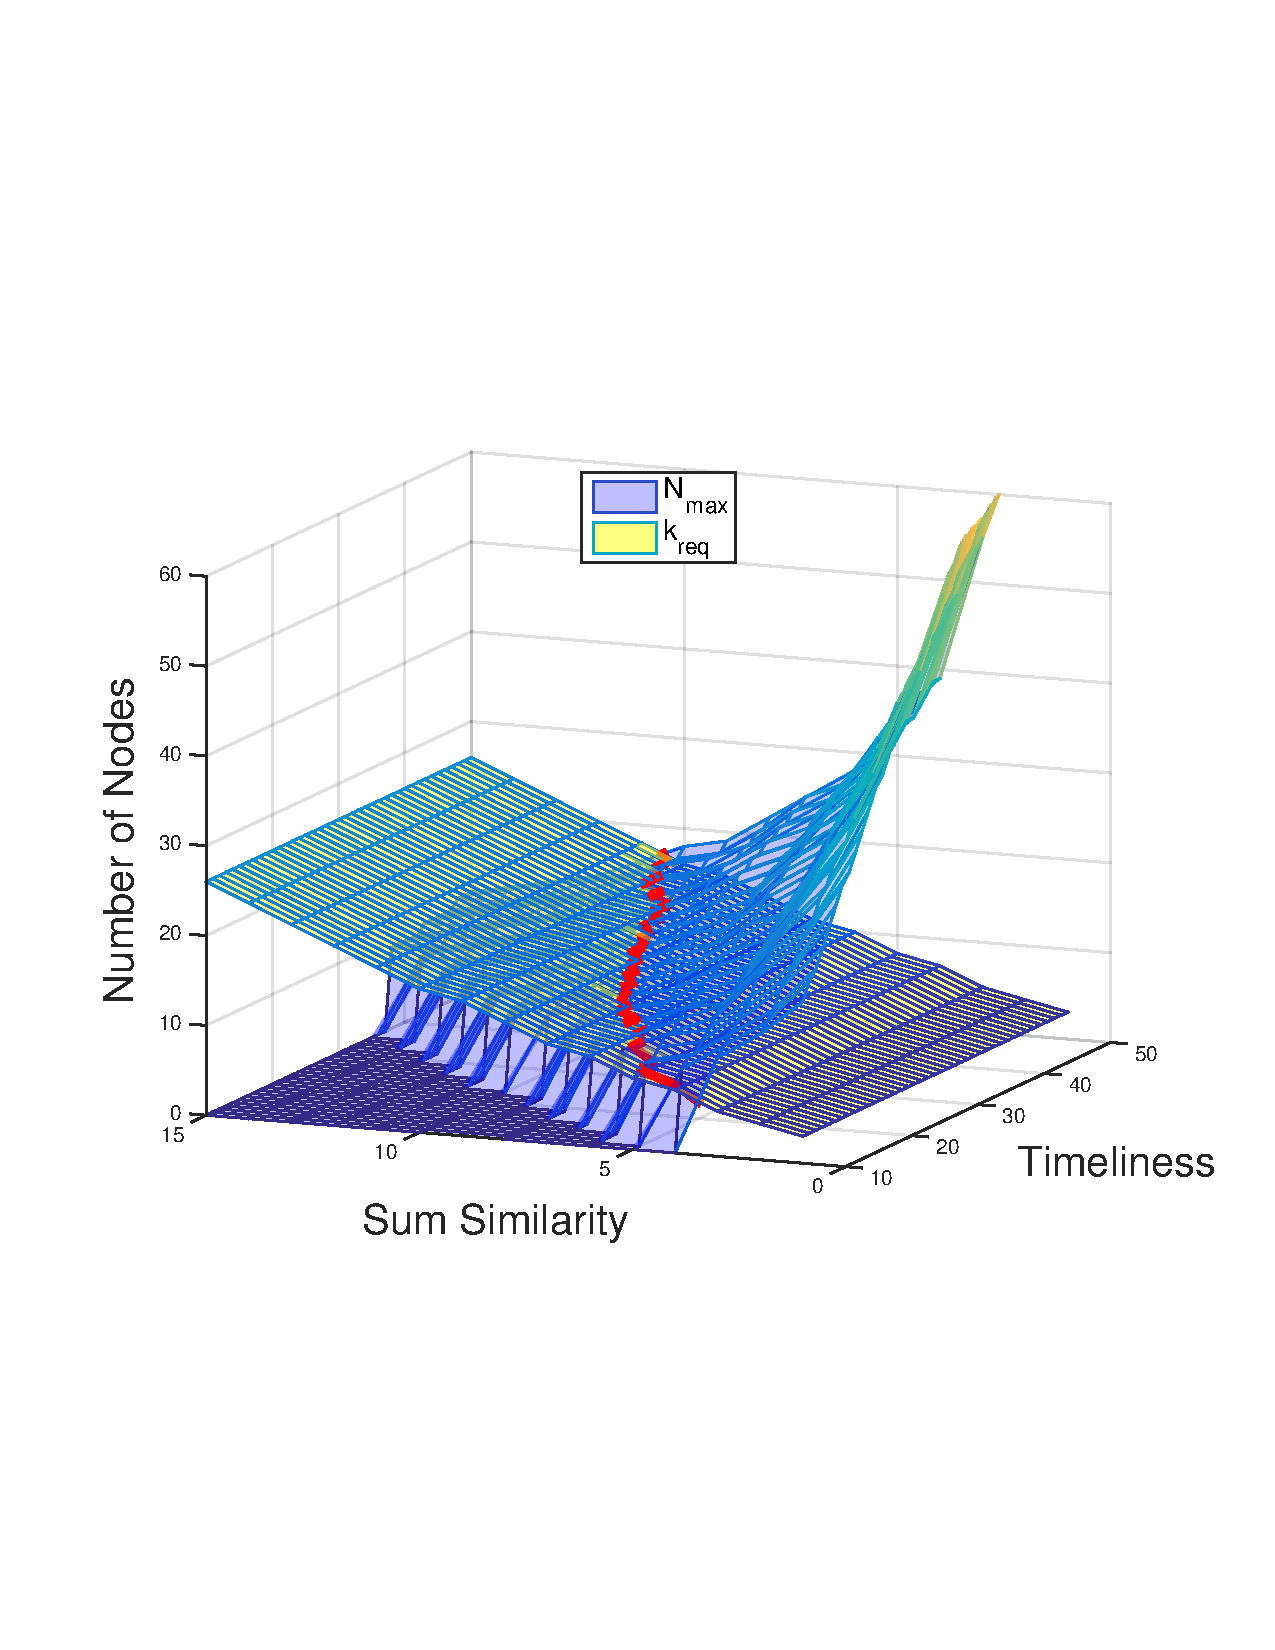
\includegraphics[scale=0.31, clip=true, trim=10mm 65mm 10mm 77mm]{figures/scal_feas_qoi/scal_feas_qoi_corner_sink_6.pdf}
		 \label{fig:scal_feasible_region_3d}
	 }
	
	\subfigure[The shaded region represents feasible values of QoI (Completeness, Timeliness pairs) - a 2-d projection from Figure \ref{fig:scal_feasible_region_3d}]
	{
		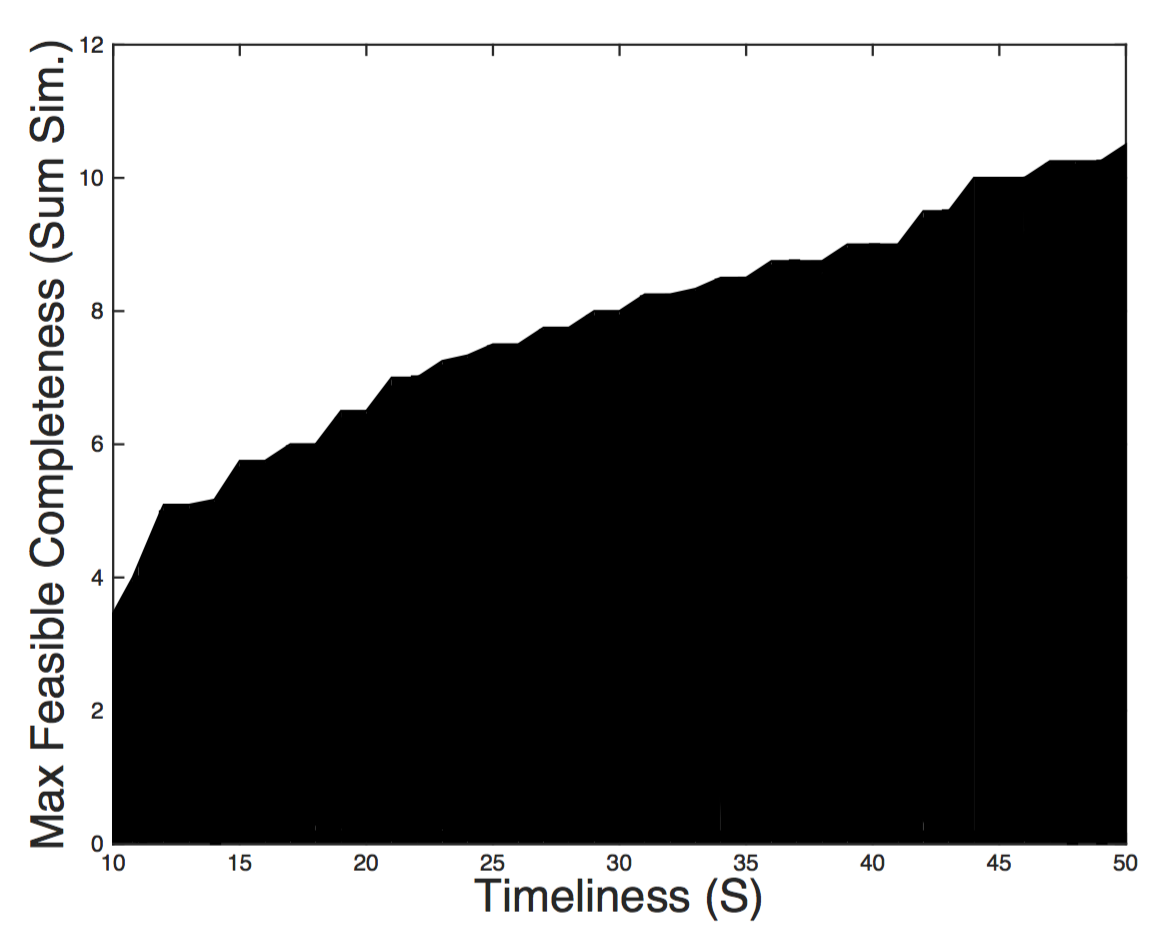
\includegraphics[scale=0.14, clip=true, trim=0mm 0mm 0mm 0mm]{figures/scal_feas_qoi/scal_feas_qoi_grid_corner_sink_2d_2.png}
		\label{fig:scal_feasible_region_2d}
	}
	\caption{Graphical representations of the \emph{Scalably Feasible QoI Region}}
	\label{fig:scal_feasible_region}
\end{figure}

Figure \ref{fig:scal_feasible_region_3d} provides a visual representation of this region for a grid network that institutes the given traffic model.
Here, $N_{max}$, calculated for QoI requirements of Sum Similarity over the range $[1, 15]$ and Timeliness over the range $[10, 50]$,
is shown in the graph by the blue surface.  On the same graph is the number of images required, $k_{req}$, for each Sum Similarity requirement, shown with the yellow surface on the graph.  The intersection of these two surfaces, displayed with a red line, provides the edge of the scalably feasible QoI region.  In this example, only QoI pairs to the right of this line, i.e. the region where $N_{max} > k_{req}$, are scalably feasible.  Figure \ref{fig:scal_feasible_region_2d} shows this same scalably feasible QoI region in two dimensions, projecting the region onto the x-y plane.  In this figure, the shaded region represents all valid pairs of completeness and timeliness requirements.

In general, regardless of how many images a node can contribute to a query response, it is possible to analyze the trade-off between different QoI attributes for a fixed value of maximum network size, $N_{max}$.  Specifically, by fixing $N$ in Table \ref{table:scal_eqs}, one can obtain $T$ and $k_{req}$ (and, hence, $C$) resulting in the set of supportable $\{C,T\}$ pairs defining a feasible region for QoI. This region can be visualized by intersecting the blue scalability curved plane with a flat surface fixed at $N_{max}$ instead of the yellow surface in Figure \ref{fig:scal_feasible_region}.  The scenario given in this section goes one step further and also takes into account  the network size actually required to generate/support a given QoI requirement (using the non-flat yellow surface derived from experimental results in Figure \ref{fig:scal_feasible_region_3d}).
